% This must be in the first 5 lines to tell arXiv to use pdfLaTeX, which is strongly recommended.
%\pdfoutput=1
% In particular, the hyperref package requires pdfLaTeX in order to break URLs across lines.

\documentclass[11pt]{article}
% Remove the "review" option to generate the final version.
\usepackage{acl}

% Standard package includes
\usepackage{times}
\usepackage{latexsym}

% For proper rendering and hyphenation of words containing Latin characters (including in bib files)
\usepackage[T1]{fontenc}
% For Vietnamese characters
% \usepackage[T5]{fontenc}
% See https://www.latex-project.org/help/documentation/encguide.pdf for other character sets

% This assumes your files are encoded as UTF8
\usepackage[utf8]{inputenc}

% This is not strictly necessary, and may be commented out,
% but it will improve the layout of the manuscript,
% and will typically save some space.
\usepackage{microtype}

% If the title and author information does not fit in the area allocated, uncomment the following
%
%\setlength\titlebox{<dim>}
%
% and set <dim> to something 5cm or larger.

%% ADDED
\usepackage{booktabs}%for table
\usepackage{multirow}
%\usepackage[table,xcdraw]{xcolor}
\usepackage{colortbl}
\usepackage{tabularx}
% from https://tex.stackexchange.com/questions/42619/xmark-that-complements-the-ams-checkmark
\usepackage{pifont}
\newcommand{\cmark}{\ding{51}}%
\newcommand{\xmark}{\ding{55}}%

%\usepackage[moderate]{savetrees}
\usepackage{graphicx}
\usepackage{tipa}


\usepackage{hyperref}
\hypersetup{
    colorlinks=true,
    linkcolor=blue,
    filecolor=magenta,      
    urlcolor=cyan,
    citecolor=black,
}
\urlstyle{same}

%% ADDED
\usepackage{wrapfig,lipsum,booktabs}

\usepackage{tikz}
%\usetikzlibrary{arrows.meta,calc,fit,positioning}
\usetikzlibrary{arrows.meta,automata,backgrounds,calc,decorations,decorations.pathmorphing,decorations.pathreplacing,fit,matrix,positioning}
\tikzset{
    invisible/.style={opacity=0},
    visible on/.style={alt={#1{}{invisible}}},
    alt/.code args={<#1>#2#3}{%
      \alt<#1>{\pgfkeysalso{#2}}{\pgfkeysalso{#3}} % \pgfkeysalso doesn't change the path
    },
}

\title{Evaluating a Phonotactic Learner for MITSL$^2_2$ Languages}


\author{Jacob K. Johnson \\
  University of Utah\\
  \small\texttt{jacob.k.johnson@utah.edu}\\
  \And 
  Aniello De Santo \\
  University of Utah\\
  \small\texttt{aniello.desanto@utah.edu}}
\begin{document}
\maketitle

\section{Introduction}
In the computational study of natural language phonotactics, work in formal language theory has highlighted subclasses of regular languages (\emph{subregular} classes) as providing insights into the fundamental properties underlying a variety of typologically attested patterns \citep{McNaughtonPapert71,chandlee2017computational}.\@
    Of particular note are Tier-based Strictly Local (TSL) languages, which capture long-distance phenomena through a formalization of the notion of phonological tier \citep{heinz2011tier}.\@ 
    Beyond typological coverage, attention has been paid recently to how observations about the subregularity of phonotactics can be tied to learnability.
    
    In this sense, grammatical inference algorithms have shown how TSL languages can be learned efficiently from positive data only \citep{jardine2016learning,jardinemcmullin17}.\@
    Additionally, super-classes of TSL have been defined to extend its typological coverage, while retaining (and improving on) its desirable (subregular) properties \citep[a.o.]{GrafMayer18}.
    
    Here, we provide an implementation of  \citet{de2021learning}'s grammatical inference learning algorithm for one such extension --- \emph{Multiple Input-sensitive Tier-based Strictly Local} languages \citep[MITSL;][]{de2019structure} --- following the standard of \emph{SigmaPie}  \citep{aksenova2020tool}\footnote{\href{https://pypi.org/project/SigmaPie/}{https://pypi.org/project/SigmaPie/}}, and evaluate it on an array of patterns with varying degrees of (subregular) complexity.\footnote{Our codebase is available \href{https://osf.io/w9prd/?view_only=d77df5dea63841fb8f749357f29df9e1}{here}.}
    
    As we illustrate below, MISTL languages are able to capture the interaction of local and non-local constraints, and while also handling multiple dependencies simultaneously.
    Their practical learnability thus has strong implications for the viability of grammatical inference/subregular approaches to phonotactic learning broadly.
    Additionally, the transparency and provable correctness of the learning algorithms developed for such formal classes can be of help in probing properties of phonotactic corpora more generally.
    

                   \begin{figure}[htbp]
    \centering
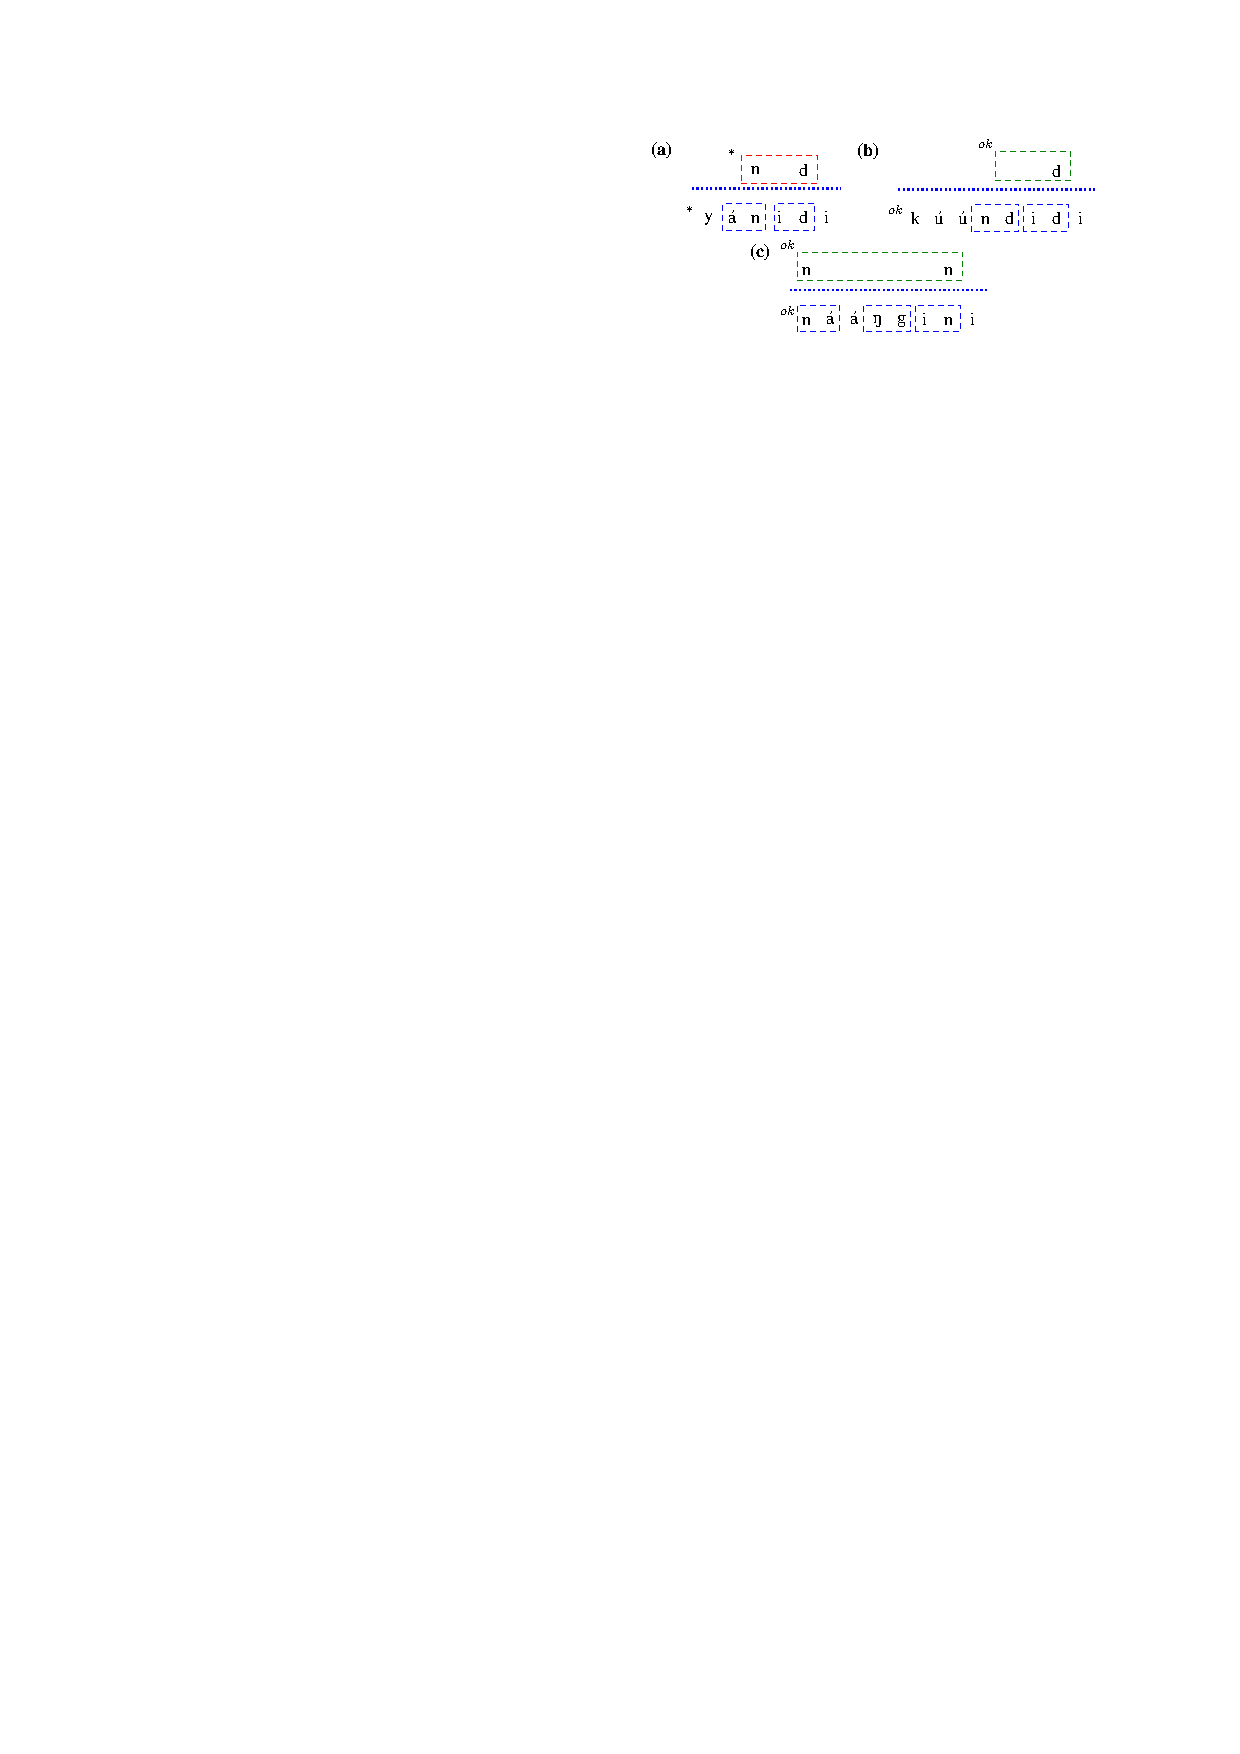
\includegraphics[width=  1\linewidth]{yaka.pdf}
\caption{ITSL$_2^2$ analysis of Yaka nasal
harmony from \citep{de2021learning}, illustrating a $2$-local projection and $2$-local tier constraints. (a) is ill-formed because of adjacent $^*$\textipa{[nd]}, but \textipa{[n,d,g,N]} are projected on the tier only when not in a nasal-stop cluster in the input (cf.\ (b), (c)).}
\label{fig:yaka}
\end{figure}
    
\section{MITSL}

TSL grammars encode long-distance dependencies by enforcing local constraints over a subset of segments in the input alphabet (the tier) identified via a projection function.\
While TSL covers many unbounded phonotactic patterns, past work has highlighted two limits: 1) since TSL's tier projection is only sensitive to properties of individual segments, it cannot handle cases where local and non-local requirements interact; 2) TSL's  reliance on a single tier (i.e.,\ lack of intersection closure) makes it unable to handle multiple non-interacting dependencies.\@
MITSL languages \citep{de2019structure} address these issues thanks to:\
\begin{enumerate}
\item an \emph{input-sensitive} (ITSL) projection, sensitive not only to a segment by itself but also to its \emph{context} in the input string (Fig.\ \ref{fig:yaka}); 
\item closure under intersection (MTSL): \emph{multiple projection functions} (tiers) are available, each with its dedicated local constraints.
\end{enumerate}


Essentially, an ITSL projection is an input strictly local function \cite{ChandleeHeinz18}, such that projection is decided by whether a segment belong to the tier alphabet, and by its immediately adjacent segment.
The MTSL component makes it so each string is evaluated on any number of distinct tier, and wellformedness is guaranteed if and only if the string is wellformed on each individual tier simultaneously.
       
 \section{Learning MITSL$^2_2$ Patterns}
\citet{de2021learning} propose a learning algorithm for MITSL$^2_2$ languages, where the tier projection and the tier constraints are bounded to bigrams (MITSL2IA),  extending \citet{McMullinSCIL2019}'s algorithm for MTSL$^2_2$ languages.\@ 

Consistently with \citep{McMullinSCIL2019}, MITSL2IA builds on the intuition that  if a bigram $\rho_1\rho_2$ is banned on some tier, then it will never appear in string-adjacent contexts. 
For each $\rho_1\rho_2$ absent from the training data, the goal is therefore to determine which segments
can be safely removed from the associated tier. To do so, the algorithm incorporates the
notion of a 2-path \citep{JardineHeinz16}.
 Intuitively, a 2-path can be thought of as a
precedence relation $(\rho_1 \dots \rho_2 )$ accompanied by the set $X$ of symbols that intervene between $\rho_1$ and $\rho_2$.
 Formally, each 2-path is therefore a 3-tuple of the form $\langle \rho_1, X, \rho_2 \rangle$. 

%For example, thestring abcc includes the following 2-paths: ha, ;, bi,ha, {b}, ci,ha, {b, c}, ci,hb, ;, ci,hb, {c}, ci.
In short, by examining the set of 2-paths present in the training data, we can determine
which segments are freely distributed with respect to a bigram $\rho_1\rho_2$ that is known to be
banned on some tier. 
%Specifically, if all of the attested h⇢1, X, ⇢2i 2-paths that include an intervening  are likewise attested without an intervening , the algorithm removes  from the tier, since the presence of ⇢1 ... ⇢2 is not dependent on an intervening .
By associating each potential bigram constraint to a specific tier, MITSL2IA is thus able to handle multiple tier projections.
In addition, \citet{de2021learning} handle the extended input contexts by generalizing the definition of tier symbols from segments to bigrams.\@
Each tier-bigram $\rho_1\rho_2$ is thus a 4-factor for MITSL2IA, such that the algorithm can evaluate a target element $\sigma$ and its left or right local context \citep[see][for technical details]{de2021learning}.
%
%All local 4-factors over the the alphabet of the input are generated, and ones that are attested in the input samples are filtered out, leaving only unattested 4-factors. It is assumed that these 4-factors are unattested because they are ungrammatical.
%For each unnatested 4-factor $a$:
%	Let $a_1$ and $a_2$ be 2-factors such that $a$ is the concatenation of $a_1$ and $a_2$:
%	It is initially known that the tier on which it is prohibited consists of at least $a_1$ and $a_2$.
%	Let $A$ be the set of sets of 2-factors found to occur between $a_1$ and $a_2$ in the sample. The ordered triple $(a_1, A, a_2)$ is referred to as a "path" in De Santo & Aksënova (2021).
%		For example: if $a =$ "wxyz" (so $a_1 =$ "wx" and $a2 =$ "yz") and there is some string "wxuvyz" in the input, then the path $("wx", \{ "xu", "uv", "vy" \}, "yz") \in A$, along with any other "paths" that occur in the input sample.
%	For each 2-factor $\beta$ over the alphabet:
%		Let $B \subseteq A$ consist of all sets in $A$ which contain $\beta$
%		Let $B'$ be formed by removing $\beta$ from every set in $B$
%		Only if $B' \subseteq A$, then $\beta$'s intervening between $a_1$ and $a_2$ has $\beta$ been shown to not be required for their long-distance grammaticality, and it is not added to the tier, otherwise it is added to the tier. 

Consistently with other work of this type, MITSL2IA is \emph{guaranteed} to learn target grammars efficiently (polynomial in time and data) in the limit, \emph{if} the input sample is \emph{characteristic} --- it contains all the information necessary to distinguish the specific target pattern(s)  \citep{Higuera2010grammatical}.
This property of learning algorithms in this tradition makes them not only valuable from a theoretical perspective, but it also allows us to use them for a deeper exploration of how target phenomena of interest are represented in data sets of different kind.
In this work, we start pursuing questions in this direction, with a preliminary investigation of the practical efficacy of \citet{de2021learning}'s learner.

%\section{Algorithm and Implementation}
 %   \paragraph{} Below is a short explanation of the algorithm; see \citet{de2021learning} for details.
   % \begin{enumerate}
   %     \item all $m \cdot k$-factors over the alphabet of the input that are not attested in the input are generated (where $m$ is the width, in segments, of a tier symbol and $k$ is the width of segment interactions)
     %   \item for each unattested $m \cdot k$ factor, it is initially assumed that the tier on which this is prohibited consists of all possible $m$-factors
     %%   \item for a given unattested $m \cdot k$ factor $a$, let $A$ be the set of sets of $m$-factors found to intervene in $a$ (also called "paths" (THIS IS NOT QUITE THE SAME TERMINOLOGY AS USED BEFORE, IS IT CLOSE ENOUGH?): for example with $m=2, k=2$: if $a=$"wxyz" and there is some string "wxuvyz" in the input, then the path $\{ "xu", "uv", "vy" \} \in A$. For any $m$-factor $\beta$, let $B \subseteq A$ be all sets in $A$ which contain $\beta$. Let $B'$ be formed by removing $\beta$ from every set in $B$. If $B' \subseteq A$, then $\beta$ has been shown to have no effect on $a$, so it is known to not be part of the tier restricting $a$.
   % \end{enumerate}
   % \paragraph{} A few notes relating to this implementation of the algorithm:
    %\begin{itemize}
    %    \item The linked implementation allows for $m=2$ and $k=2$ only (MITSL$_2^2$). These windows are large enough to capture all the patterns mentioned above.
     %   \item For computational efficiency, the assumptions of steps 2 and 3 were results were inverted, that is, tier were assumed to be empty each 2-factors was added to a tier if it could not be concluded that that 2-factor was not on that tier.
     %   \item A special case must be implemented to prevent overlapping $m$-factors from triggering a restriction.
    %\end{itemize}
    
     \begin{figure}[t]
     \centering
                  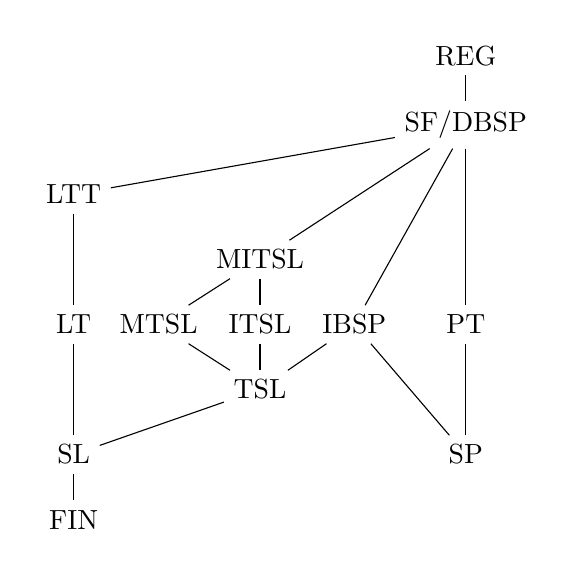
\begin{tikzpicture}
                    \node (m) at (0,0) [matrix of nodes, ampersand replacement=\&,
                                        row sep=1em] {%
                           \&       \&       \&           \&      \& REG\\
                           \&       \&       \&           \&      \& SF/DBSP\\
                           \& LTT   \\
                           \&       \&       \& MITSL\\
                           \& LT    \& MTSL  \& ITSL    \& IBSP \& PT\\
                         \&       \&  \& TSL\\
                           \& SL    \&       \&           \&      \& SP\\
                           \& FIN\\
                    };
                    \foreach \Source/\Target in {%
                        1-6/2-6,
                        2-6/3-2,
                        2-6/4-4,
                        2-6/5-5,
                        2-6/5-6,
                        3-2/5-2,
                        4-4/5-3,
                        4-4/5-4,
                        5-2/7-2,
                        5-3/6-4,
                        5-4/6-4,
                        5-5/6-4,
                        5-5/7-6,
                        5-6/7-6,
                      %  6-3/7-2,
                        6-4/7-2,
                        7-2/8-2%
                        }
                        \draw (m-\Source) to (m-\Target);
                \end{tikzpicture}
 \caption{Subsumption of subregular classes, with the TSL extensions as of \citep{de2019structure}.}
\label{fig:subregular}
  \end{figure}
    
\begin{table}[t!]
\centering
\resizebox{0.5\textwidth}{!}{%
\begin{tabular}{|cccccc|}
\hline
\multicolumn{1}{|c|}{}                   & \multicolumn{4}{c|}{Aks{\"e}nova (2020)}      & \multicolumn{1}{|c|}{This Paper}                                                                                                                                                                                                          \\ \cline{2-6}
\multicolumn{1}{|c|}{\multirow{-2}{*}{}} & \multicolumn{1}{c|}{SP}                            & \multicolumn{1}{c|}{SL}                            & \multicolumn{1}{c|}{TSL}                           & \multicolumn{1}{c|}{MTSL}                          & MITSL                         \\ \hline
\multicolumn{6}{|c|}{Word-final devoicing}                                                                                                                                                                                                                                                   \\ \hline
\multicolumn{1}{|c|}{T}                  & \multicolumn{1}{c|}{{\color[HTML]{FE0000} \xmark}} & \multicolumn{1}{c|}{{\color[HTML]{548235} \cmark}} & \multicolumn{1}{c|}{{\color[HTML]{548235} \cmark}} & \multicolumn{1}{c|}{{\color[HTML]{548235} \cmark}} & {\color[HTML]{548235} \cmark} \\ \hline
\multicolumn{1}{|c|}{A}                  & \multicolumn{1}{c|}{\cellcolor[HTML]{F8CBAD}68\%}  & \multicolumn{1}{c|}{\cellcolor[HTML]{548235}100\%} & \multicolumn{1}{c|}{\cellcolor[HTML]{548235}100\%} & \multicolumn{1}{c|}{\cellcolor[HTML]{548235}100\%} & \cellcolor[HTML]{548235}100\% \\ \hline
\multicolumn{1}{|c|}{N$_1$}                  & \multicolumn{1}{c|}{\cellcolor[HTML]{F8CBAD}58\%}  & \multicolumn{1}{c|}{\cellcolor[HTML]{548235}100\%} & \multicolumn{1}{c|}{\cellcolor[HTML]{548235}100\%} & \multicolumn{1}{c|}{\cellcolor[HTML]{548235}100\%} & \cellcolor[HTML]{548235}100\% \\ \hline
\multicolumn{6}{|c|}{Single vowel harmony without blocking}                                                                                                                                                                                                                                  \\ \hline
\multicolumn{1}{|c|}{T}                  & \multicolumn{1}{c|}{{\color[HTML]{548235} \cmark}} & \multicolumn{1}{c|}{{\color[HTML]{FE0000} \xmark}} & \multicolumn{1}{c|}{{\color[HTML]{548235} \cmark}} & \multicolumn{1}{c|}{{\color[HTML]{548235} \cmark}} & {\color[HTML]{548235} \cmark} \\ \hline
\multicolumn{1}{|c|}{A}                  & \multicolumn{1}{c|}{\cellcolor[HTML]{548235}100\%} & \multicolumn{1}{c|}{\cellcolor[HTML]{F8CBAD}83\%}  & \multicolumn{1}{c|}{\cellcolor[HTML]{548235}100\%} & \multicolumn{1}{c|}{\cellcolor[HTML]{548235}100\%} & \cellcolor[HTML]{548235}100\% \\ \hline
\multicolumn{1}{|c|}{N$_2$}                  & \multicolumn{1}{c|}{\cellcolor[HTML]{548235}100\%} & \multicolumn{1}{c|}{\cellcolor[HTML]{F8CBAD}72\%}  & \multicolumn{1}{c|}{\cellcolor[HTML]{548235}100\%} & \multicolumn{1}{c|}{\cellcolor[HTML]{548235}100\%} & \cellcolor[HTML]{548235}100\% \\ \hline
\multicolumn{6}{|c|}{Single vowel harmony with blocking}                                                                                                                                                                                                                                     \\ \hline
\multicolumn{1}{|c|}{T}                  & \multicolumn{1}{c|}{{\color[HTML]{FE0000} \xmark}} & \multicolumn{1}{c|}{{\color[HTML]{FE0000} \xmark}} & \multicolumn{1}{c|}{{\color[HTML]{548235} \cmark}} & \multicolumn{1}{c|}{{\color[HTML]{548235} \cmark}} & {\color[HTML]{548235} \cmark} \\ \hline
\multicolumn{1}{|c|}{A}                  & \multicolumn{1}{c|}{\cellcolor[HTML]{F8CBAD}84\%}  & \multicolumn{1}{c|}{\cellcolor[HTML]{F8CBAD}89\%}  & \multicolumn{1}{c|}{\cellcolor[HTML]{548235}100\%} & \multicolumn{1}{c|}{\cellcolor[HTML]{548235}100\%} & \cellcolor[HTML]{C6E0B4}99\%  \\ \hline
\multicolumn{6}{|c|}{Several vowel harmonies without blocking}                                                                                                                                                                                                                               \\ \hline
\multicolumn{1}{|c|}{T}                  & \multicolumn{1}{c|}{{\color[HTML]{548235} \cmark}} & \multicolumn{1}{c|}{{\color[HTML]{FE0000} \xmark}} & \multicolumn{1}{c|}{{\color[HTML]{548235} \cmark}} & \multicolumn{1}{c|}{{\color[HTML]{548235} \cmark}} & {\color[HTML]{548235} \cmark} \\ \hline
\multicolumn{1}{|c|}{A}                  & \multicolumn{1}{c|}{\cellcolor[HTML]{548235}100\%} & \multicolumn{1}{c|}{\cellcolor[HTML]{F8CBAD}69\%}  & \multicolumn{1}{c|}{\cellcolor[HTML]{548235}100\%} & \multicolumn{1}{c|}{\cellcolor[HTML]{548235}100\%} & \cellcolor[HTML]{548235}100\% \\ \hline
\multicolumn{6}{|c|}{Several vowel harmonies with blocking}                                                                                                                                                                                                                                  \\ \hline
\multicolumn{1}{|c|}{T}                  & \multicolumn{1}{c|}{{\color[HTML]{FE0000} \xmark}} & \multicolumn{1}{c|}{{\color[HTML]{FE0000} \xmark}} & \multicolumn{1}{c|}{{\color[HTML]{548235} \cmark}} & \multicolumn{1}{c|}{{\color[HTML]{548235} \cmark}} & {\color[HTML]{548235} \cmark} \\ \hline
\multicolumn{1}{|c|}{A}                  & \multicolumn{1}{c|}{\cellcolor[HTML]{F8CBAD}76\%}  & \multicolumn{1}{c|}{\cellcolor[HTML]{F8CBAD}59\%}  & \multicolumn{1}{c|}{\cellcolor[HTML]{548235}100\%} & \multicolumn{1}{c|}{\cellcolor[HTML]{548235}100\%} & \cellcolor[HTML]{C6E0B4}99\%  \\ \hline
\multicolumn{1}{|c|}{N$_3$}                  & \multicolumn{1}{c|}{\cellcolor[HTML]{F8CBAD}76\%}  & \multicolumn{1}{c|}{\cellcolor[HTML]{F8CBAD}70\%}  & \multicolumn{1}{c|}{\cellcolor[HTML]{F8CBAD}67\%}  & \multicolumn{1}{c|}{\cellcolor[HTML]{C6E0B4}95\%}  & \cellcolor[HTML]{C6E0B4}99\%  \\ \hline
\multicolumn{6}{|c|}{\begin{tabular}[c]{@{}c@{}}Vowel harmony and consonant \\ harmony without blocking\end{tabular}}                                                                                                                                                                        \\ \hline
\multicolumn{1}{|c|}{T}                  & \multicolumn{1}{c|}{{\color[HTML]{548235} \cmark}} & \multicolumn{1}{c|}{{\color[HTML]{FE0000} \xmark}} & \multicolumn{1}{c|}{{\color[HTML]{FE0000} \xmark}} & \multicolumn{1}{c|}{{\color[HTML]{548235} \cmark}} & {\color[HTML]{548235} \cmark} \\ \hline
\multicolumn{1}{|c|}{A}                  & \multicolumn{1}{c|}{\cellcolor[HTML]{548235}100\%} & \multicolumn{1}{c|}{\cellcolor[HTML]{F8CBAD}64\%}  & \multicolumn{1}{c|}{\cellcolor[HTML]{F8CBAD}74\%}  & \multicolumn{1}{c|}{\cellcolor[HTML]{548235}100\%} & \cellcolor[HTML]{548235}100\% \\ \hline
\multicolumn{6}{|c|}{\begin{tabular}[c]{@{}c@{}}Vowel harmony and consonant \\ harmony with blocking\end{tabular}}                                                                                                                                                                           \\ \hline
\multicolumn{1}{|c|}{T}                  & \multicolumn{1}{c|}{{\color[HTML]{FE0000} \xmark}} & \multicolumn{1}{c|}{{\color[HTML]{FE0000} \xmark}} & \multicolumn{1}{c|}{{\color[HTML]{FE0000} \xmark}} & \multicolumn{1}{c|}{{\color[HTML]{548235} \cmark}} & {\color[HTML]{548235} \cmark} \\ \hline
\multicolumn{1}{|c|}{A}                  & \multicolumn{1}{c|}{\cellcolor[HTML]{F8CBAD}83\%}  & \multicolumn{1}{c|}{\cellcolor[HTML]{F8CBAD}64\%}  & \multicolumn{1}{c|}{\cellcolor[HTML]{F8CBAD}69\%}  & \multicolumn{1}{c|}{\cellcolor[HTML]{548235}100\%} & \cellcolor[HTML]{548235}100\% \\ \hline
\multicolumn{6}{|c|}{Unbounded tone plateauing}                                                                                                                                                                                                                                              \\ \hline
\multicolumn{1}{|c|}{T}                  & \multicolumn{1}{c|}{{\color[HTML]{548235} \cmark}} & \multicolumn{1}{c|}{{\color[HTML]{FE0000} \xmark}} & \multicolumn{1}{c|}{{\color[HTML]{FE0000} \xmark}} & \multicolumn{1}{c|}{{\color[HTML]{FE0000} \xmark}} & {\color[HTML]{548235} \cmark} \\ \hline
\multicolumn{1}{|c|}{A}                  & \multicolumn{1}{c|}{\cellcolor[HTML]{548235}100\%} & \multicolumn{1}{c|}{\cellcolor[HTML]{F8CBAD}85\%}  & \multicolumn{1}{c|}{\cellcolor[HTML]{F8CBAD}90\%}  & \multicolumn{1}{c|}{\cellcolor[HTML]{BFBFBF}}      & \cellcolor[HTML]{548235}100\% \\ \hline
\multicolumn{6}{|c|}{\begin{tabular}[c]{@{}c@{}}Two locally-driven long-distance\\ assimilations (ITSL restrictions)\end{tabular}}                                                                                                                                                           \\ \hline
\multicolumn{1}{|c|}{T}                  & \multicolumn{1}{c|}{{\color[HTML]{FE0000} \xmark}} & \multicolumn{1}{c|}{{\color[HTML]{FE0000} \xmark}} & \multicolumn{1}{c|}{{\color[HTML]{FE0000} \xmark}} & \multicolumn{1}{c|}{{\color[HTML]{FE0000} \xmark}} & {\color[HTML]{548235} \cmark} \\ \hline
\multicolumn{1}{|c|}{A}                  & \multicolumn{1}{c|}{\cellcolor[HTML]{BFBFBF}}      & \multicolumn{1}{c|}{\cellcolor[HTML]{BFBFBF}}      & \multicolumn{1}{c|}{\cellcolor[HTML]{BFBFBF}}      & \multicolumn{1}{c|}{\cellcolor[HTML]{BFBFBF}}      & \cellcolor[HTML]{548235}100\% \\ \hline
\end{tabular}
}
\caption{(T)heoretical expectations and performance of $5$ subregular learners on (A)rtificial and simplified (N)atural language input data-sets.\ MITSL corresponds to the learner evaluated in this paper. N$_1$: German;  N$_1$: Finnish;  N$_1$: Turkish.}
\label{tbl:languages}
\vspace{-0.5cm}
\end{table}
%\section{Evaluating MITSL2IA}

\section{Evaluating MITSL2IA}
    We implemented MITSL2IA in Python 3 following requirements of the \emph{SigmaPie} toolkit, and evaluated it  over patterns resembling natural language phenomena belonging to different subregular classes, according to the pipeline argued for by \citet{aksenova2020tool}.\@
    
    The learner had as input datasets which were either the artificial outputs of harmonic string generators incorporating a target grammar, or natural language word-lists with simplified alphabets created by masking ``irrelevant'' symbols \cite[for details see][]{aksenova2020tool}. 
    Each artificial dataset contained $1000$ randomly sampled strings, and up to $130K$ words for the simplified natural language corpora.\@
  
    MITSL2IA's output grammars were then used as input to string generators.\@
    We evaluated the \emph{consistency} of the learned grammar with respect to the target grammar, by computing the number of strings in the newly generated sample that were well-formed according to the target generalization ($\%$ of new strings accepted by the original grammar).\@
  
  Following  \citep{aksenova2020tool}, we included patterns from subclasses of MITSL which are also known to be attested in natural languages (cf. Fig.\ \ref{fig:subregular} and Tbl.\ref{tbl:languages}).
  An unbounded tone-plateauing pattern \citep{hyman2010tone,Jardine16} characterized as Strictly Piecewise (SP)  in past literature also served as a simple ITSL pattern \citep{de2019structure}, and we added an explicitly MITSL pattern not included in \citep{aksenova2020tool}.
        The performance of our implementation on each dataset was compared to what reported by \citet[][]{aksenova2020tool} for a battery of other subregular learners (Tbl.\ \ref{tbl:languages}).\@
    %proposes to evaluate grammatical inference algorithms not on how a learned grammar classifies a held out set (as is a more traditional machine-learning approach), but rather by sampling strings from the learned grammar and then determining how many and which of them are accepted by the target grammar. This approach verifies grammar consistency rather than completeness, which is important given the nature of the algorithm, which essentially is the process of explaining a restriction on all unattested $m*k$-factors: if a particular restriction has not been learned, or has been learned incorrectly (An $m$-factor failed to be removed from a tier), then the learned grammar will accept strings form outside of the target grammar.
    % In \citet{aksenova2020tool}, learning algorithms for all language classes in Table 1 (except MITSL) were evaluated on all the patterns described in Table 1 (except two intertwined ITSL restrictions, which was first performed in \citealt{de2021learning}). This work expands on their methodology by evaluating the MITSL inference algorithm on the other patterns from \citet{aksenova2020tool}. 

   % \paragraph{} The new MITSL algorithm was applied to datasets which were either the artificial outputs of random harmonic string generators or simplified versions of natural languages, where the generation or simplification code was taken from \citet{aksenova2020tool}. For evaluations on artificial data, 1000 input strings were sampled from the harmonic string generators, while for simplified natural language experiments, the corpora contained 25K-700K words.
   % \paragraph{} The randomly generated datasets and the natural language datasets were designed to contain patterns belonging to subregular classes of languages, as shown in Table 1 (from \citealt{aksenova2020tool}, where details into the language patterns can be found). Notably, "unbounded tone plateauing" and "first-last harmony" are neither TSL or MTSL, so they could not be learned by the algorithms implemented in \citet{aksenova2020tool}. Rather, these patterns are ITSL, which is a subset of MITSL.


\section{Results and Discussion}

Recall that while MITSL2IA is guaranteed to learn a pattern when a sample is characteristic, we did not control for that requirement when generating the input datasets.
Our results show that even with small, randomly generated datasets the learner performed well on all target patterns (Tbl.\ \ref{tbl:languages}).

% Since the input samples were not tested to be ``characteristic" convergence was not guaranteed, but the learner performed well on all target patterns (Tbl.\ \ref{tbl:languages}).
     While a larger scale evaluation paradigm is an important future step, these results are encouraging in supporting the reliability of MITSL2IA in practical scenarios and highlight the importance of implementations to test grammatical inference algorithms beyond theoretical convergence.\@
  
    Importantly, since subregular classes in the TSL ``neighborhood'' stand in a subsumption relation with respect to each other (Fig.\ \ref{fig:subregular}), the learner is theoretically expected to be able to generalize correctly not only when trained on strictly MISTL patterns, but to each one of the simpler patterns as well.
 However, high-performance on subclasses of MITSL (SL, TSL, MTSL) was not trivially granted in practice.\@
    Since MITSL2IA needs evidence from all possible local contexts to recognize tier elements, it requires more evidence for simple patterns (e.g., whether to project a sibilant on a tier or not) than its less expressive counterparts.\@
    So one might expect the needed characteristic samples to be larger, when moving from simpler to more expressive learning algorithms.
    In fact, this effect is behind the slightly lower performance on the single harmony data, compared to the TSL and MTSL learners.
    %
   % 
    However, this is where the transparent nature of the algorithm shines.
    By inspecting the grammar outputted by MITSL2IA, it was possible to infer that the initial sample for those patterns lacked evidence to discard one particular element from the harmony tier.
    
    For example, the input data was insufficient for the learner to converge on the target grammar for the ``single vowel harmony with blockers'' and the ``several vowel harmonies with blocking'' cases.
    In both instances, this was because an element that should have been transparent to the restriction was not removed from the tier, because of the default assumption that all elements are on the tier restricting any unattested bigram (4-factor).
     
   To further probe the relation between algorithm convergence and information gaps in the input sample,  we thus defined an injection procedure on top of the learner itself.
   Specifically, we implemented an automatic processes to detect miscathegorized strings in the newly generated samples due an element $\beta$ that should have been removed from the tier restricting the factor $a$ as follows:
   
   \begin{enumerate}
        \item Find the set of all paths $B$ which contain $\beta$ and are attested to be interveners for $a$;
        \item Let the set $B'$ be formed by removing $\beta$ from all paths in $B$;
        \item Every path $b \in B' - A$ must be attested in the input while intervening $a$. In practice, for MITSL$_2^2$ grammars, these strings can be formed by overlapping $m$-factors in $b$, and, for $a = \alpha_1 \alpha_2$, having the string start with $\alpha_1$ and end with $\alpha_2$. Importantly, because paths are sets, $m$-factors in $b$ can be repeated.
    \end{enumerate}
   
    Re-running the learner on the injected samples resulted in a $100\%$ performance on all three of the $99\%$ cases, suggesting that transparent learners of this kind could be used to inspect the quality of the data in natural language samples available to phonotactic learners more broadly.
    Additionally, this suggests ways of expanding the current batch learning approach to MISTL data to online algorithms.
 
 \section{Conclusion}
This work adds to the theoretical contribution of \citep{de2021learning}, by showing how an implementation of their algorithm is strikingly successful on a variety of phonotactic patterns.
We also argue that the evaluation pipeline adopted here, following \citep{aksenova2020tool}, is valuable for future empirical testing of subregular learning algorithms in the grammatical inference tradition.
 
  At the same time, we suggest more broadly that implemented grammatical inference algorithms like MITSL2IA can be crucial in the future to more deeply probe how/whether sufficient information about target patterns appears in phonotactic corpora, contributing to the study of the relation between data and learning performance both in humans and machines.


\bibliography{custom,sstsl,cls2017,yale2016}
\bibliographystyle{acl_natbib}

% Annual Meeting of  the ACL

% put all citations on an extra page that will be cut out in post;
% that way we can keep using natbib commands for citations
\end{document}